
\documentclass{book}
\usepackage[utf8]{inputenc}
\usepackage{graphicx}
\usepackage{tikz}
\usepackage{float}
\usepackage{wrapfig,lipsum}
\usepackage{svg}
\usepackage{mathtools}
\usepackage{tabu}
%\usepackage{subcaption}
\usepackage{subfigure}
\usepackage[a4paper, total={6in, 8in}]{geometry}
\usepackage{minted}

\usemintedstyle{xcode}

\definecolor{bg}{rgb}{0.95,0.95,0.95}




\begin{document}


\newcommand{\vecthreeBF}[1]{\vec{\textbf{#1}}}
\newcommand{\vecthree}[1]{\vec{#1}}
\newcommand{\vecNum}[3]{(#1, #2, #3)}

\newcommand{\parDeriv}[2]{\frac{\partial #1}{\partial #2}}
\newcommand{\parDerivS}[2]{\frac{\partial^2 #1}{\partial #2^2}}
\newcommand{\derivS}[2]{\frac{d^2 #1}{d#2^2}}

\newcommand{\dotProdBF}[2]{\vecthreeBF{#1} \cdot \vecthreeBF{#2}}
\newcommand{\dotProd}[2]{\vecthree{#1} \cdot \vecthree{#2}}

\newcommand{\crossProdBF}[2]{\vecthreeBF{#1} \times \vecthreeBF{#2}}
\newcommand{\crossProd}[2]{\vecthree{#1} \times \vecthree{#2}}

\newcommand{\e}{$\textbf{e}^-$ }
\newcommand{\egun}{$\textbf{e}^-$-gun }
\newcommand{\eB}{$\textbf{e}^-$ - $\vecthreeBF{B}$ }
\newcommand{\eE}{$\textbf{e}^-$ - $\vecthreeBF{E}$ }
\newcommand{\eEM}{$\textbf{e}^-$ - \textbf{EM} }
\newcommand{\ee}{$\textbf{e}^-$ - $\textbf{e}^-$ }


\newcommand{\fromeq}[1]{\textit{equation \ref{eq:#1}}}
\newcommand{\fromeqs}[2]{\textit{equations \ref{eq:#1} and \ref{eq:#2}}}
\newcommand{\fromeqsth}[3]{\textit{equations \ref{eq:#1}, \ref{eq:#2} and \ref{eq:#3}}}
\newcommand{\fromeqsf}[4]{\textit{equations \ref{eq:#1}, \ref{eq:#2}, \ref{eq:#3} and \ref{eq:#4}}}

\newcommand{\fromfig}[1]{\textit{figure \ref{fig:#1}}}
\newcommand{\fromfigs}[2]{\textit{figures \ref{fig:#1} and \ref{fig:#2}}}
\newcommand{\fromfigf}[4]{\textit{figures \ref{fig:#1}, \ref{fig:#2}, \ref{fig:#3} and \ref{fig:#4}}}

\newcommand{\fromsec}[1]{\textit{section \ref{sec:#1}}}
\newcommand{\fromsecs}[2]{\textit{sections \ref{sec:#1} and \ref{sec:#2}}}

\newcommand{\fromapp}[1]{\textit{Appendix \ref{appendix:#1}}}

\newcommand{\fromtab}[1]{\textit{Table \ref{tab:#1}}}
\newcommand{\fromtabs}[2]{\textit{Tables \ref{tab:#1} and \ref{tab:#2}}}



%----../../..++++.

%%%%%%
% Start of intermediate.tex
\clearpage
\section{Graphical User Interface}

Until this point, \textit{Rhodotron Simulation} could be used with a configration file, defining the problem that would be simulated.
An example of this configuration file can be found in \fromfig{config_file} of \fromapp{example_simulation_runs}. 
\vspace{10pt}
\begin{figure}[H]
    \centering
    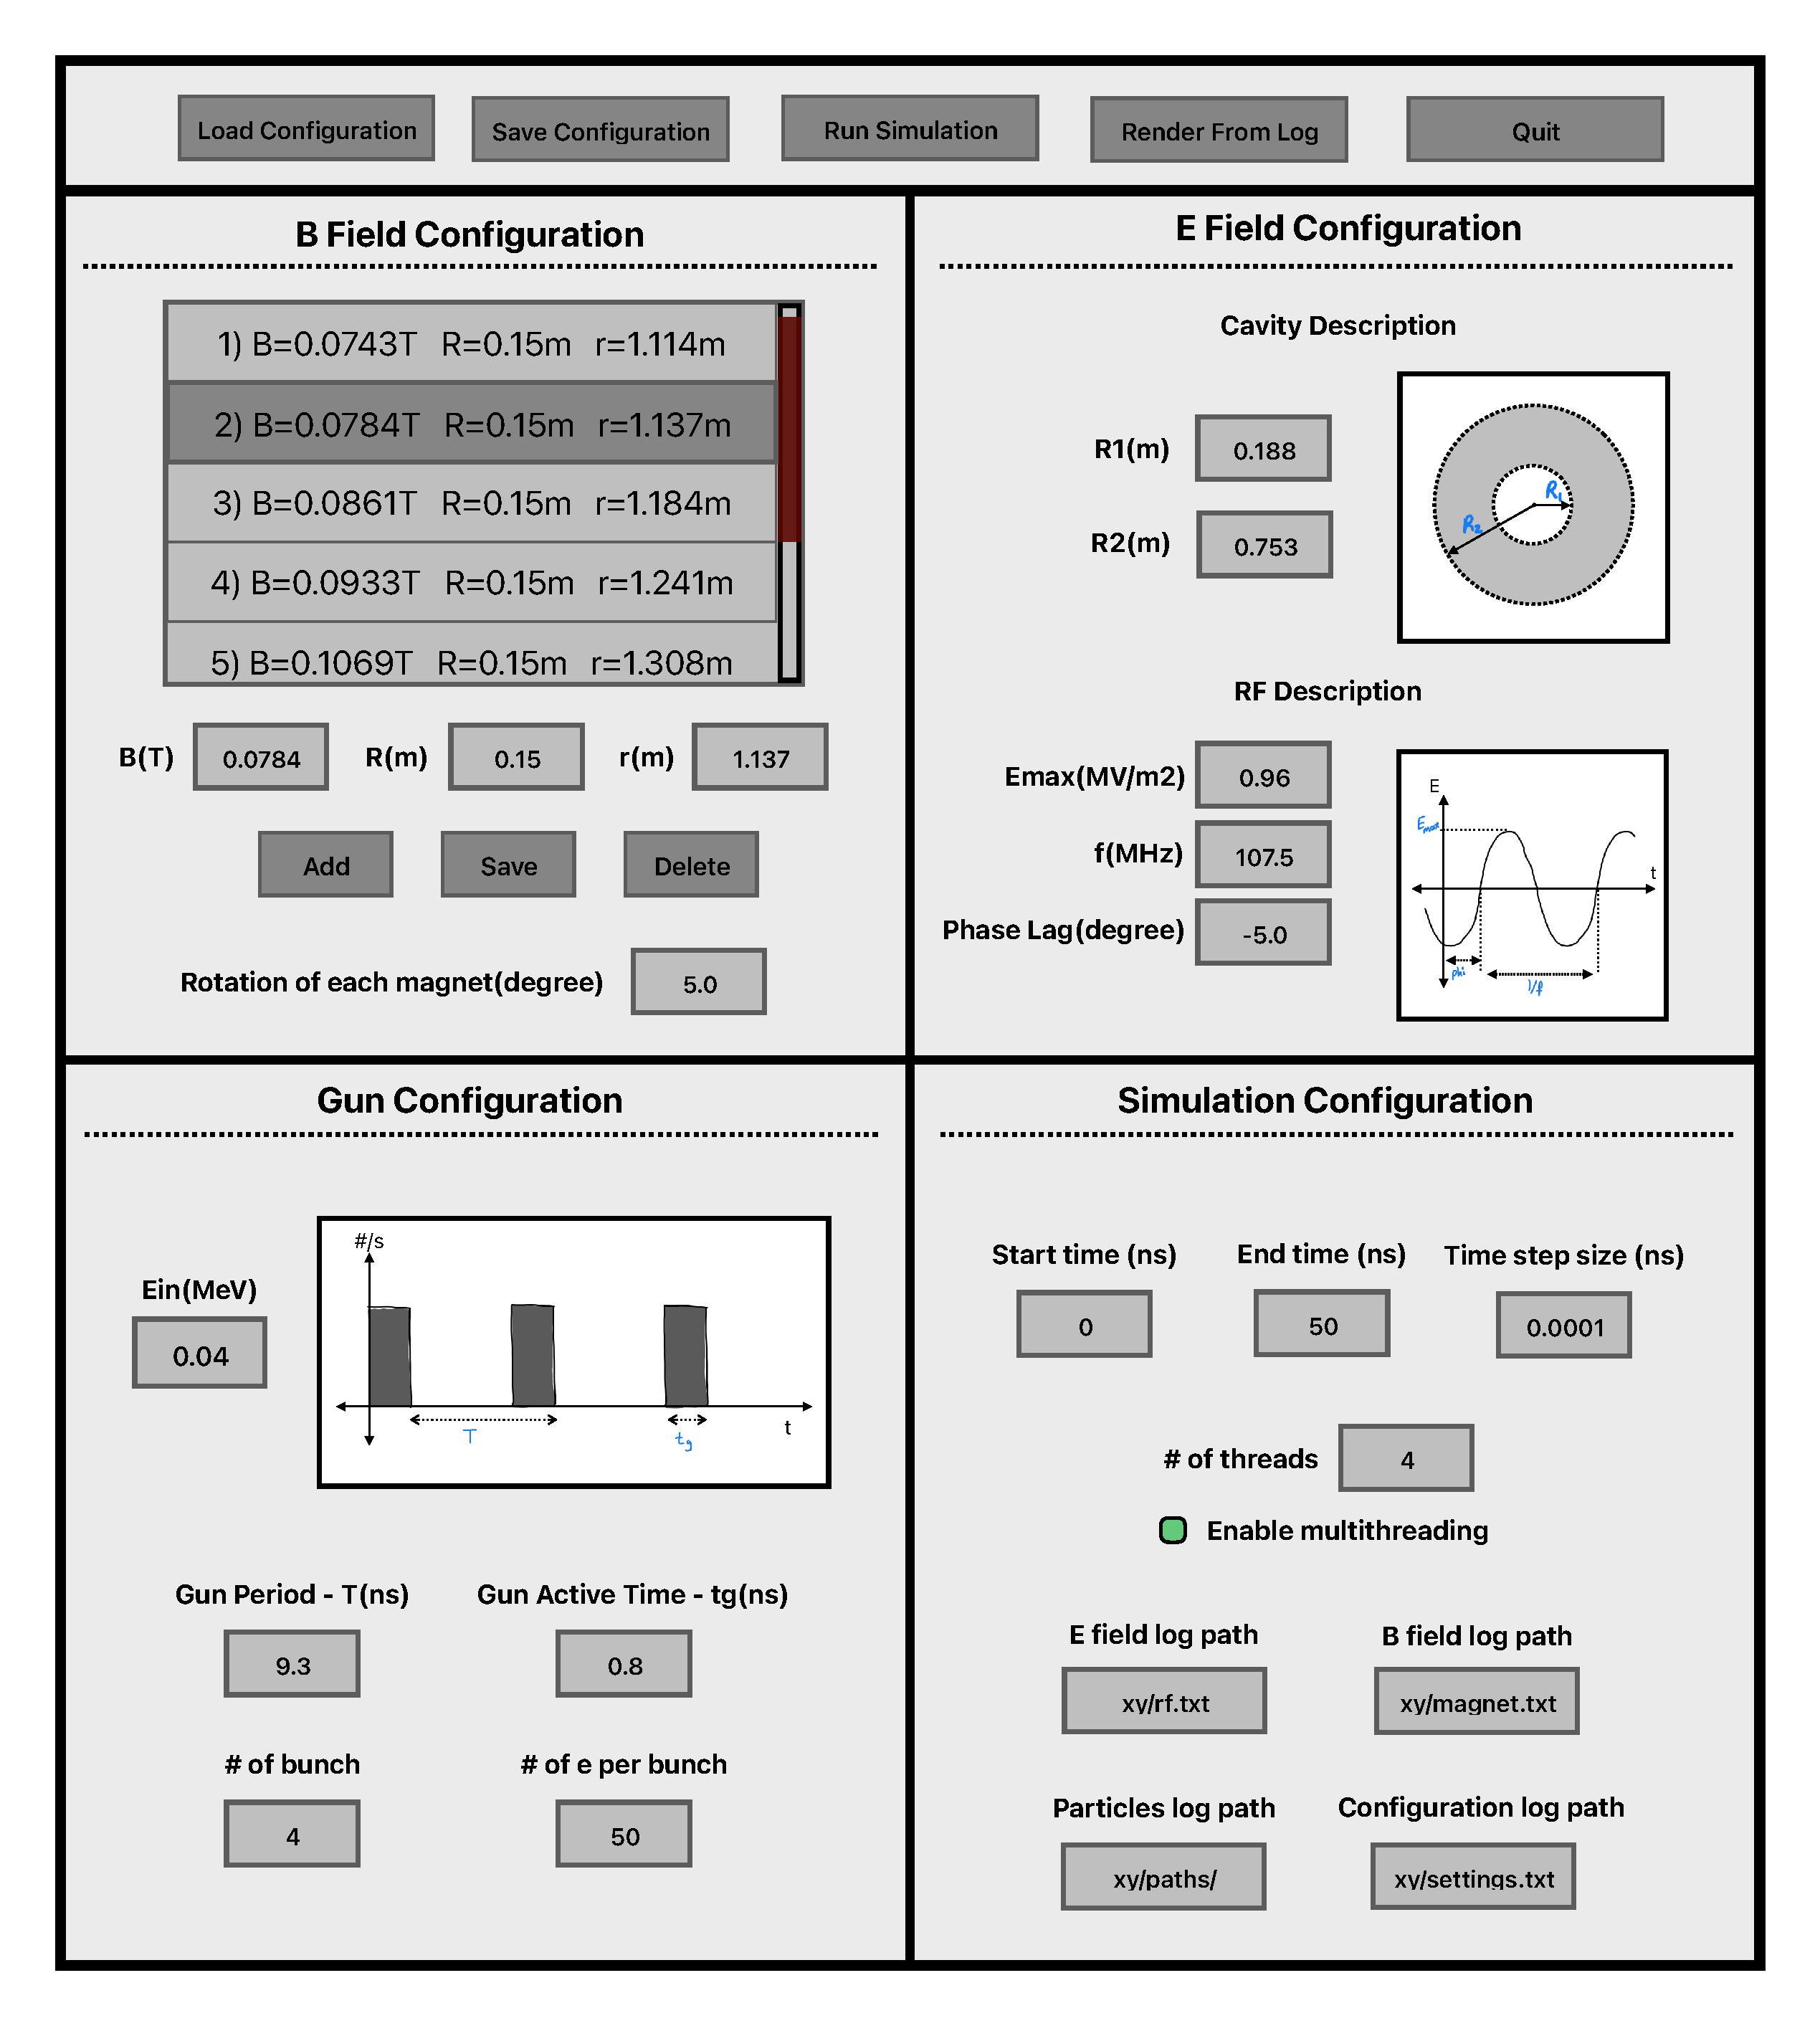
\includegraphics[width=\linewidth]{../../../figures/illustrations/RhodoSim_GUI_Draft_V02.pdf}
    \caption{An Illustration of the first GUI design.}
    \label{fig:gui_illustration}
\end{figure}
\clearpage
This approach was simple and fast; however, it was not suitable for the average target user since required basic knowledge of command line interface and was not up to modern standards.
For this reason, a GUI was decided to be built, using \textit{ROOT framework}. 
This would also enable \textit{Rhodotron simulation} to make use of analysis tools offered by \textit{ROOT}.

The initial design of the \textit{Rhodotron Simulation GUI} can be observed in \fromfig{gui_illustration}.
The \textit{GUI} would be a standalone application, running the \textit{Rhodotron Simulation} as a service when needed. 
For this reason, the now called \textit{simulation engine} was updated to be able to run as a background service of \textit{GUI}.
By this approach, one could also ignore the \textit{GUI} altogether and use the \textit{simulation engine} as before, as these are two seperate products.

In the \fromfig{gui_config}, the implemented version of \fromfig{gui_illustration} can be observed. 
Available frames of this version of the \textit{GUI} are discussed further in the following sections.
\subsection{Simulation Frame}
This frame spawns and manages the \textit{simulation engine}, configures and starts the simulation. 
It has a progress bar that shows the current progress of the simulation, communucating with \textit{UI handler thread} in \textit{simulation engine}.
Simulation frame while a simulation is running can be observed in \fromfig{gui_simulate_1} of \fromapp{supp}.
\clearpage
\subsection{Configuration Frame}
This frame provides an interface for specifying, saving or loading a configuration, consists of $\vecthreeBF{B}$ field, $\vecthreeBF{E}$ field, \textit{RF} description, \egun, \textit{simulation} configuration regions.
Each one having an illustration of what the parameters are as can be seen in \fromfig{gui_config}.
\vspace{10pt}
\begin{figure}[h]
    \centering
    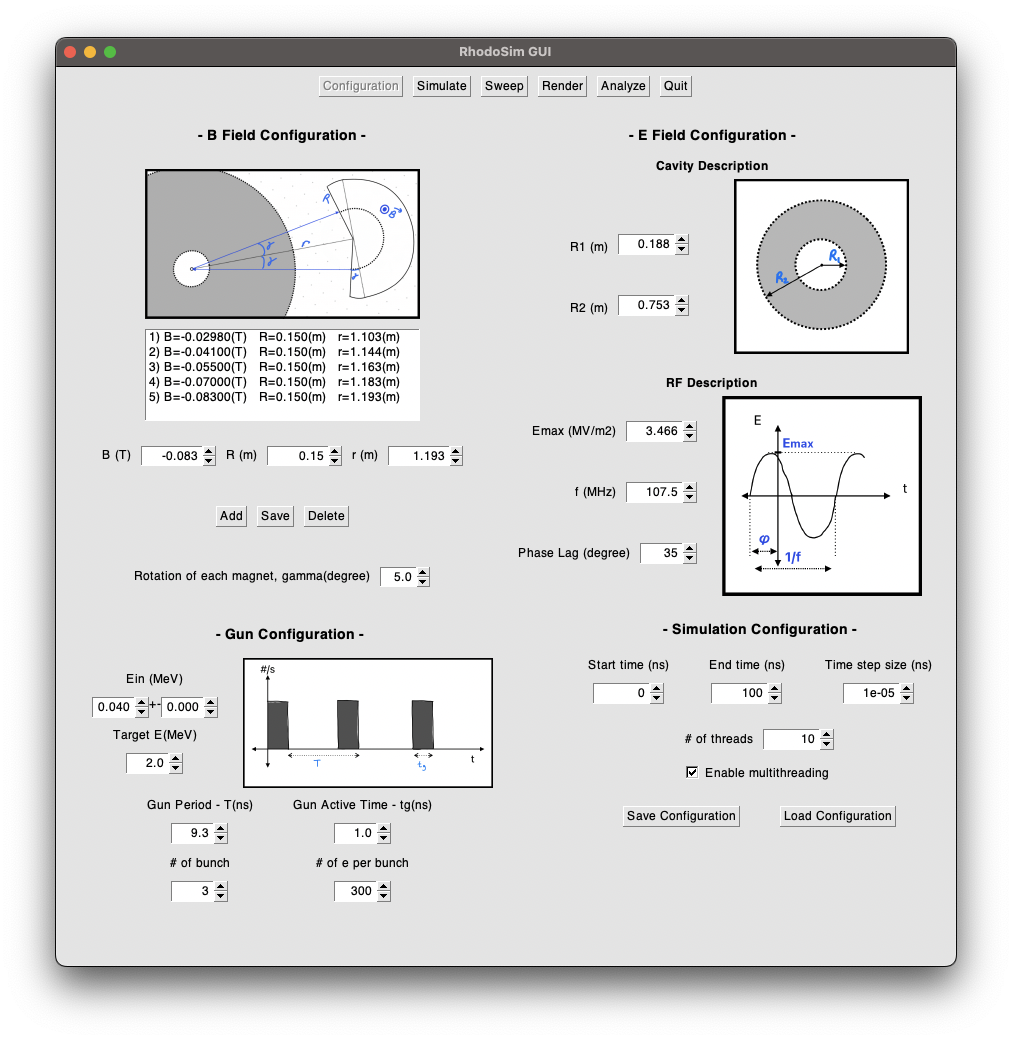
\includegraphics[width=\linewidth]{../../../figures/rhodoSim/GUI_config_frame.png}
    \caption{The configuration frame of implementated first GUI design.}
    \label{fig:gui_config}
\end{figure}

\clearpage
\subsection{Render Frame}
Since the rendering capabilities of \textit{ROOT} is superior than \textit{gnuplot}, the user can render a playback of the simulation in real time, 
see a specific time frame, export as snapshot or animated gif file.
Two example renders can be seen in \fromfig{gui_render_1} and \fromfig{gui_render_2} of \fromapp{supp}.
\vspace{10pt}
\begin{figure}[h]
    \centering
    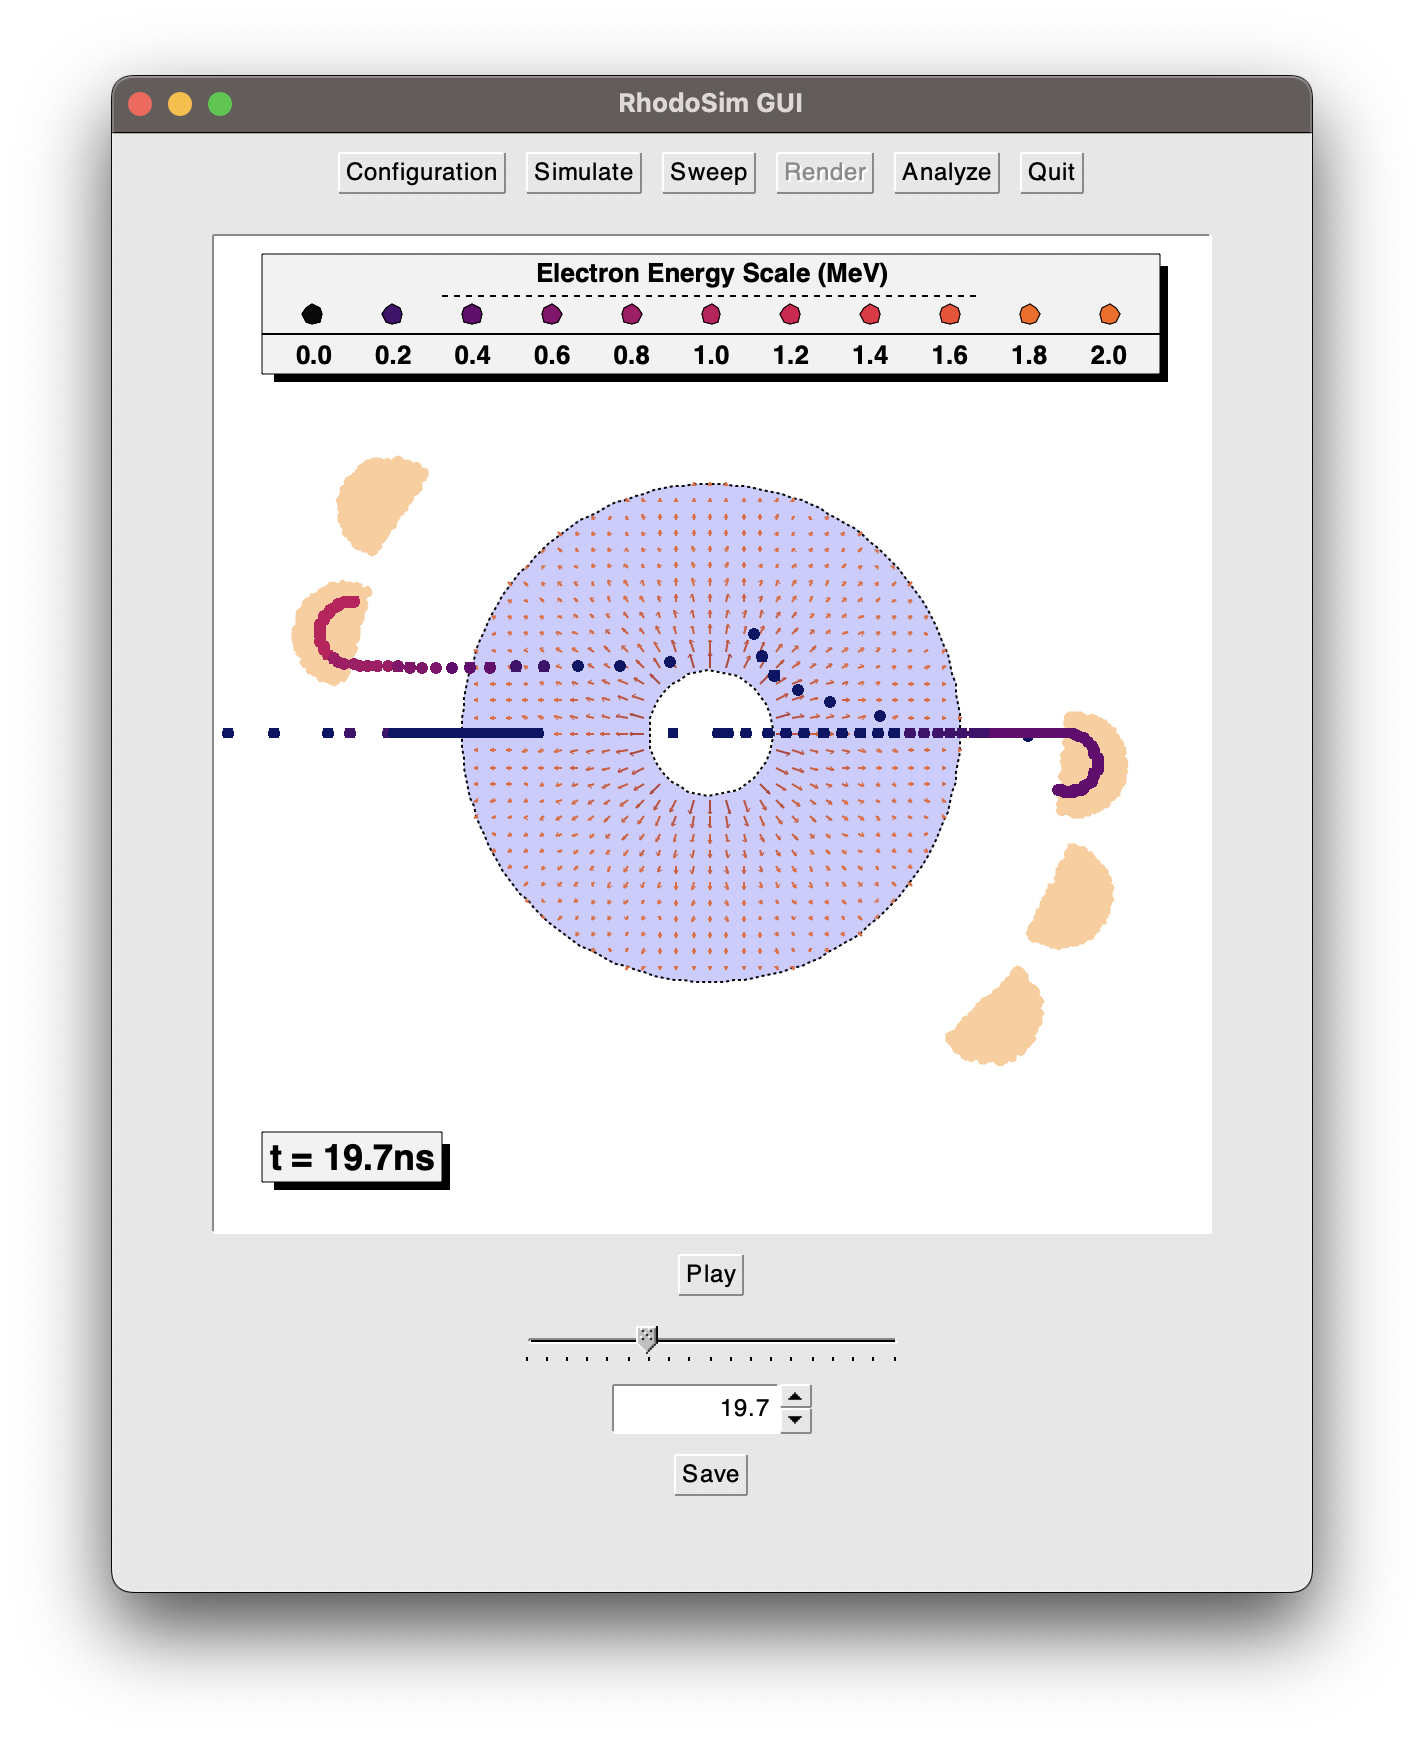
\includegraphics[width=0.85\linewidth]{../../../figures/rhodoSim/GUI_render_frame_5.png}
    \caption{Render frame of \textit{GUI}.}
    \label{fig:gui_render_1}
\end{figure}

\subsection{Analyze Frame}
Analyze frame provides tools for analyzing and visualizing the simulation data. 
In the current version, energy distribution histogram and \textit{E(t)} graph of each electron are implementated into this frame.
This frame is a work in progress and will be the focus of improvement and become a really powerfull tool in the near future.
In \fromfig{gui_analyze_Edist}, \textit{Analyze Frame} plotting energy distribution histogram, and in \fromfig{gui_analyze_Et} and \fromfig{gui_analyze_Et2} of \fromapp{supp}, \textit{Analyze Frame} plotting \textbf{E(t)} graphs can be observed.
\vspace{10pt}
\begin{figure}[h!]
    \centering
    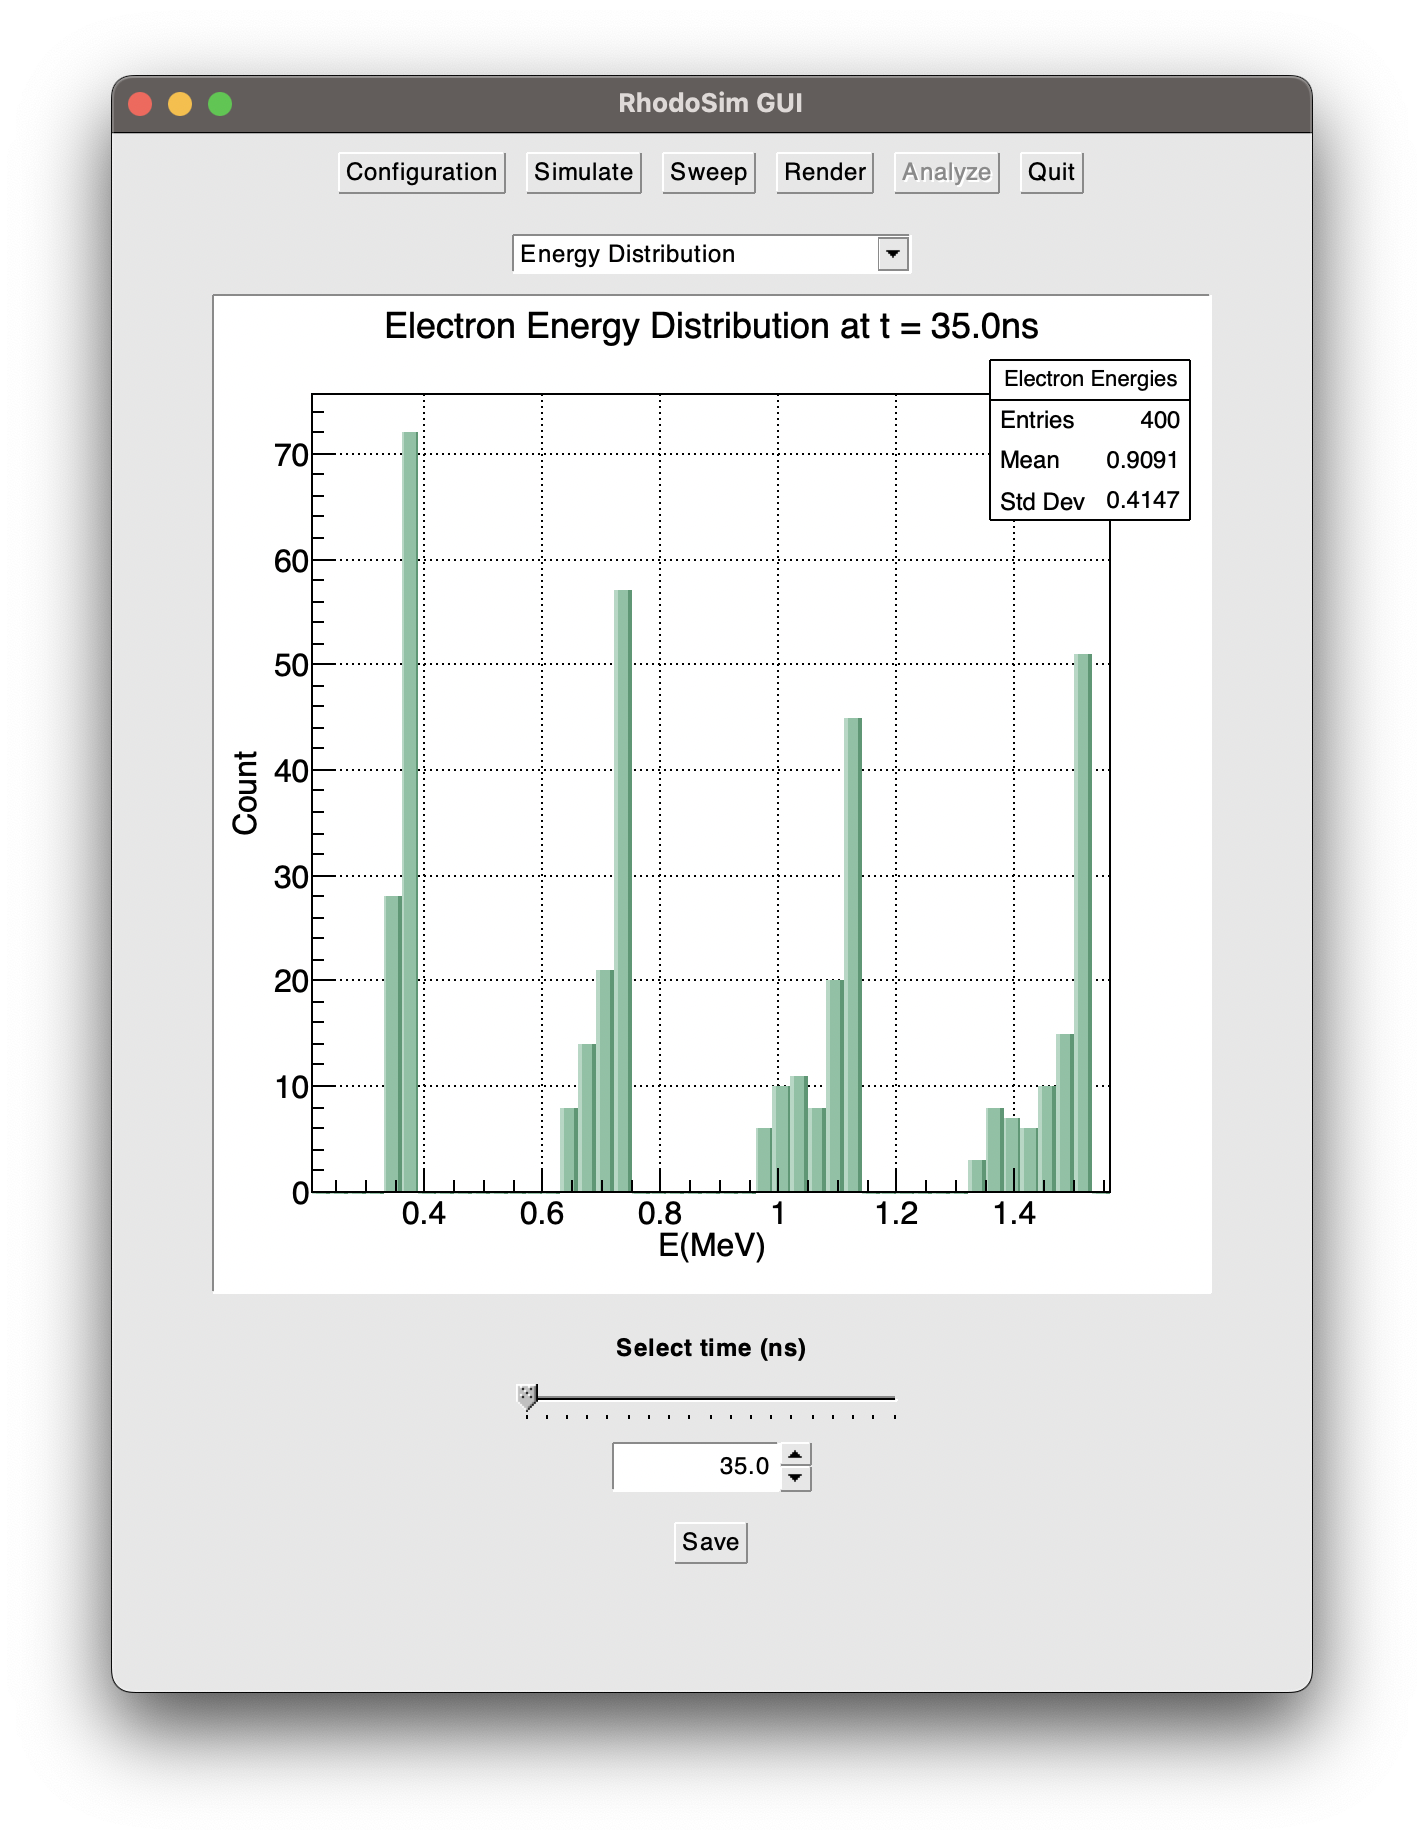
\includegraphics[width=0.8\linewidth]{../../../figures/rhodoSim/GUI_analyze_Edist_2.png}
    \caption{Analyze frame of \textit{GUI} E distribution.}
    \label{fig:gui_analyze_Edist}
\end{figure}

\begin{figure}[h!]
    \centering
    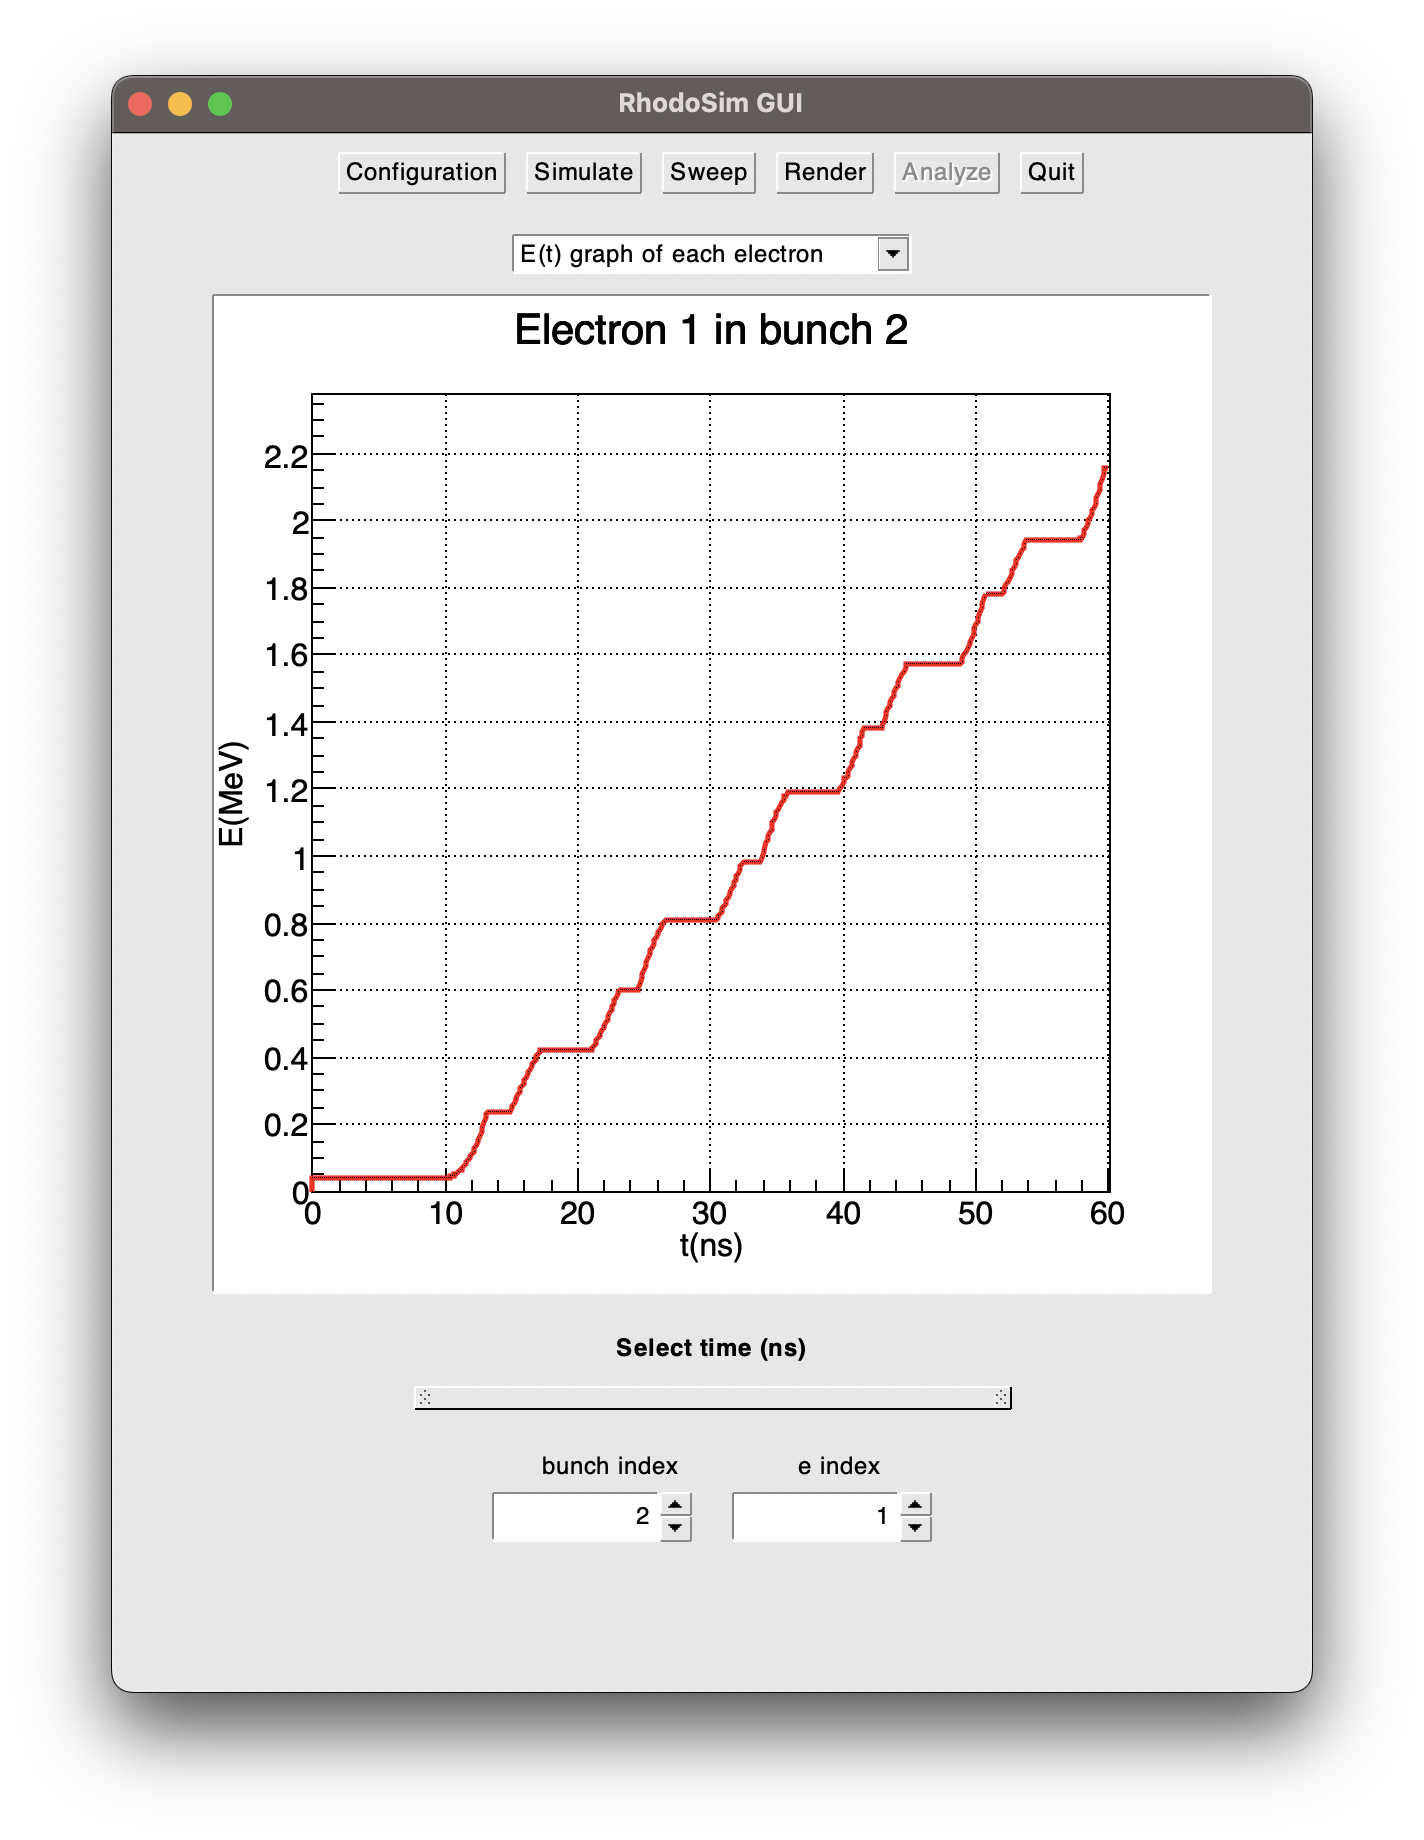
\includegraphics[width=0.9\linewidth]{../../../figures/rhodoSim/GUI_analyze_Et_3.png}
    \caption{Analyze frame of \textit{GUI} E(t).}
    \label{fig:gui_analyze_Et}
    \vspace{20pt}
\end{figure}

\subsection{Sweep Frame}
Parameter sweep method that was discussed in \fromsecs{lout_sweep}{philag_sweep} was integrated into \textit{GUI} in a seperate frame named \textit{Sweep Frame}.
$\phi_{lag}$ sweep was the first parameter to be implemented. 

It takes the range of sweep, draws $\phi_{lag}$ vs $\mu E$, $\phi_{lag}$ vs $\sigma E$ and $\phi_{lag}$ vs $\sigma R$ mentioned in \fromsec{philag_sweep}.
This enables user with an already built accelerator to optimize \egun parameters quickly. 
In the \fromfigf{gui_sweep_muE}{gui_sweep_sE}{gui_sweep_running}{gui_sweep_sR} of \fromapp{supp}, this frame can be inspected in detail.
\vspace{10pt}
\begin{figure}[h]
    \centering
    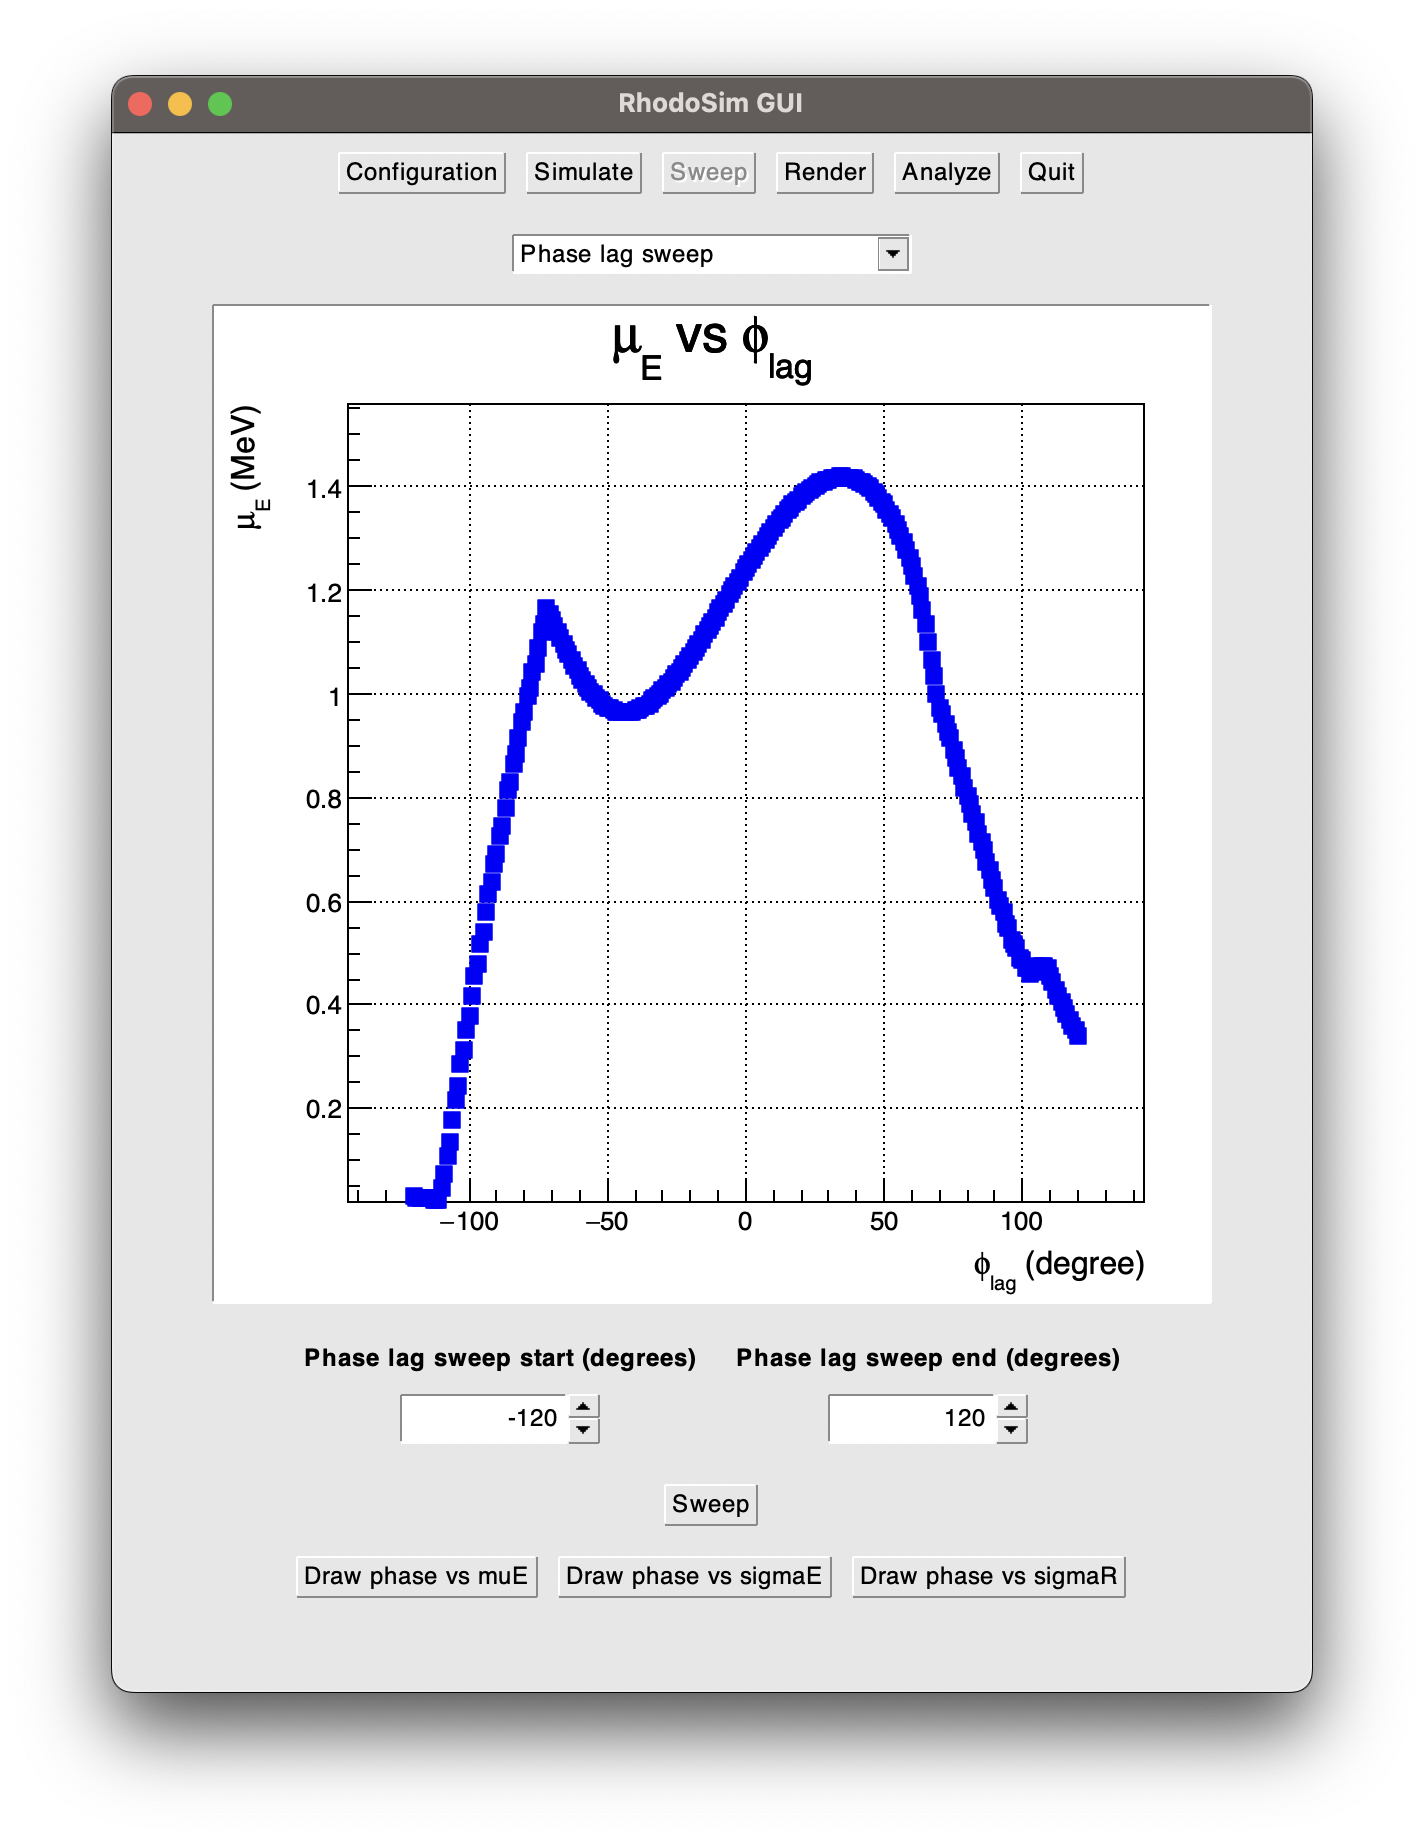
\includegraphics[width=0.85\linewidth]{../../../figures/rhodoSim/GUI_sweep_muE_3.png}
    \caption{Sweep frame of \textit{GUI} $\phi_{lag}$ $\mu E$ result.}
    \label{fig:gui_sweep_muE}
\end{figure}
\clearpage
\begin{figure}[h]
    \centering
    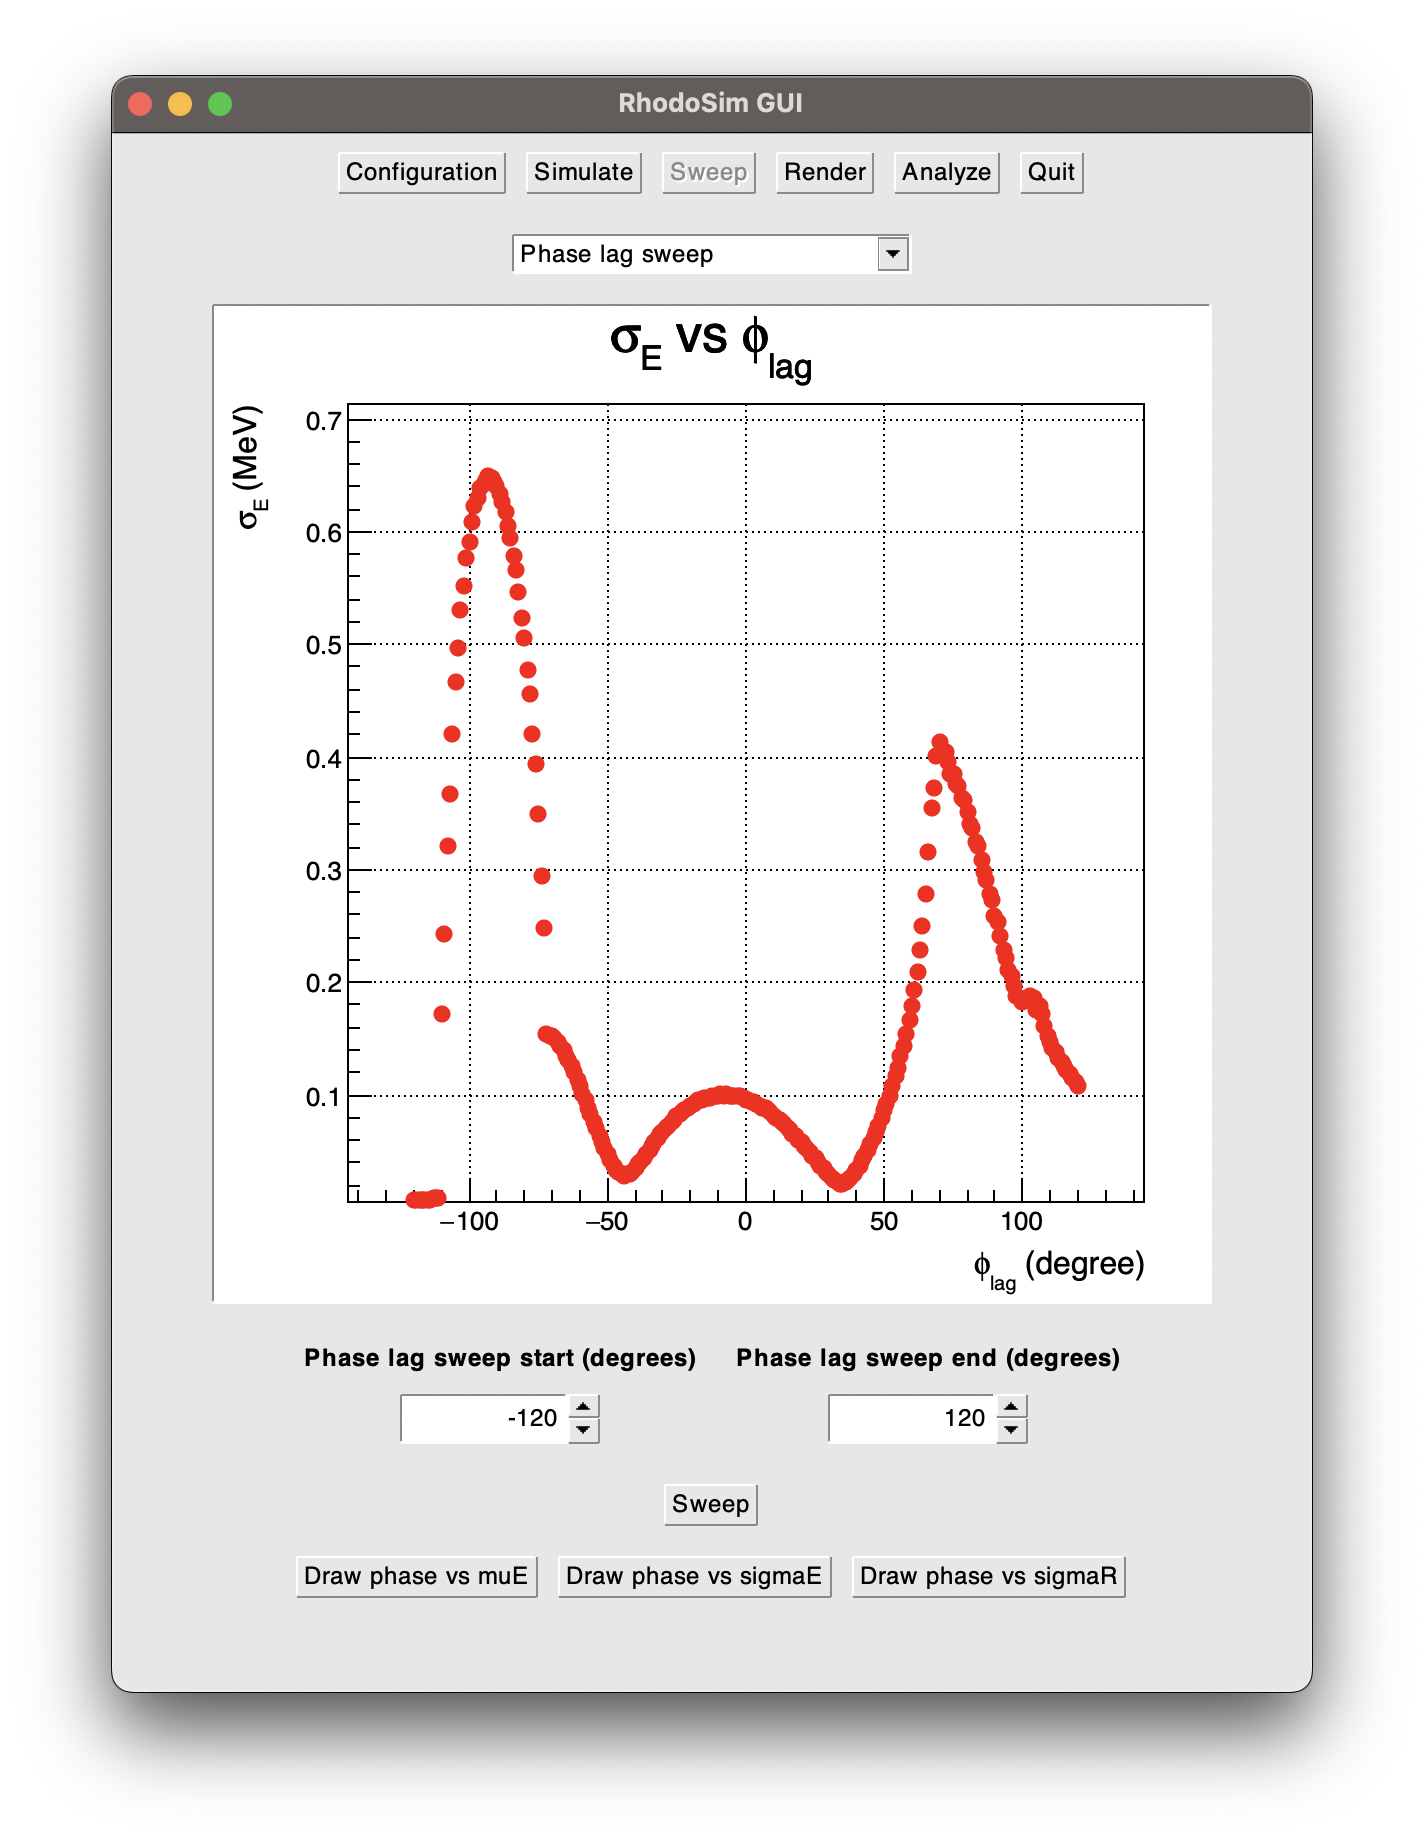
\includegraphics[width=0.85\linewidth]{../../../figures/rhodoSim/GUI_sweep_sE_3.png}
    \caption{Sweep frame of \textit{GUI} $\phi_{lag}$ sweep $\sigma E$ result.}
    \label{fig:gui_sweep_sE}
    \vspace{10pt}
\end{figure}

As mentioned before, \textit{GUI} is the latest and ongoing development effort in this project.
New analysis and sweep features will be implemented and current capabilities will be improved in the near future.

%%%%%%


\end{document}